\chapter{Perancangan}
\label{chap: perancangan}
	
	Pada bab ini akan dijelaskan mengenai perancangan aplikasi yang dibangun meliputi perancangan kelas, \textit{routes}, \textit{controllers}, \textit{models}, perancangan antarmuka.
	
	\section{Perancangan Kelas}
	\label{sec: rancangKelas}
	
	Seperti yang sudah di jelaskan pada bab sebelumnya, untuk memodelkan sistem penilaian sidang skripsi 2 dengan menggunakan \textit{codeigniter} membutuhkan \textit{routes}, \textit{controllers}, \textit{models}, dan \textit{views}. Hal-hal berikut akan dijelaskan pada subbab selanjutnya.
	
	\section{Routes}
	\label{sec: routes}
	
	\textit{Routes} merupakan bagian dari \textit{codeigniter} untuk melakukan pemetaan terhadap lokasi \textit{file controllers} dari aplikasi. Berikut adalah isi dari "config/routes":
	\begin{lstlisting}
		$route['default_controller'] = 'C_skripsi';
		$route['404_override] ="";
		$route[translate_url_dahses'] =	FALSE;
	\end{lstlisting}
	Baris pertama dari kode di atas adalah nama \textit{file controller} yang terletak di \textit{folder controllers} yang akan diambil. Baris kedua merupakan kode untuk menangani \textit{error} yang terjadi jika \textit{file} yang dicari tidak ditemukan, contoh penggunaanya adalah "\$route['404\_override'] = 'errors/page\_missing;". Baris ketiga mempunyai fungsi mengganti seluruh nama \textit{file} yang mengandung '-' menjadi '\_', contoh penggunaanya adalah: "my-controller/index"	menjadi "my\_controller/index".

	\section{Controllers}
	\label{sec: controllers}
	
	\textit{Controller} terdiri dari sebuah kelas yang dinamakan "C\_Skripsi". Keseluruhan aktivitas dari sistem informasi penilaian skripsi diatur oleh kelas ini. Berikut adalah gambar kelas diagram dari \textit{controllers}:
	\begin{figure}[H]
		\centering
		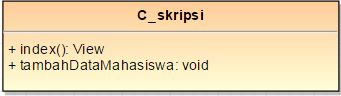
\includegraphics[scale= 1.0]{Gambar/C_skripsi}
		\caption {Gambar diagram kelas \textit{file controllers}}
		\label{fig:controllers}
	\end{figure}
	
	\begin{itemize}
		\item public function index()
		Berfungsi untuk mengarahkan pengguna ke \textit{file views default} dari aplikasi.
		\item public function tambahDataMahasiswa()
		Berfungsi untuk mengambil data dari \textit{view} yang tersedia, untuk kemudian diolah menjadi bahasa sql oleh \textit{models}.
	\end{itemize}
	
	\section{Models}
	\label{sec: models}
	
	\textit{Models} mempunyai fungsi menghubungkan \textit{views} dan \textit{controllers} pada basis data. Pada penggunaan \textit{codeigniter}, \textit{model} dibuat dengan sangat sederhana. Berikut adalah isi dari kelas model:
	\begin{lstlisting}
		<?php
			defined('BASEPATH') OR exit('No direct script access allowed');
			
			class Skripsi_model extends CI_Model {
			
			public function insertDataMahasiswa($tableName, $data){
				$res = $this->db->insert($tableName, $data);
			}
		}
		
	\end{lstlisting}
	
	\begin{itemize}
		\item public function insertDataMahasiswa(\$tablename, \$data)
		Berfungsi untuk mengolah data yang sudah diolah oleh \textit{controllers} menjadi kueri sql \textit{insert data}.
	\end{itemize}
	
	\section{Perancangan Basis Data}
	\label{sec: perancanganDatabase}
	
	Berdasarkan analisis basis data pada bab \ref{sub: analisisDatabase}, maka dibuat tabel basis data berisi:
	
	\begin{tabular}{| m{0.75cm} | m{7cm} | m{3cm} |}
		\hline
		No & Nama Tabel & Jenis Data\\
		\hline
		1 & \underline{id} & int(11)\\
		\hline
		2 & tahun & year(4)\\
		\hline
		3 & semester & int(1)\\
		\hline
		4 & npm & varchar(10)\\
		\hline
		5 & nama & varchar(256)\\
		\hline
		6 & judul & varchar(256)\\
		\hline
		7 & namaPembimbing & varchar(256)\\
		\hline
		8 & namaPembimbingPendamping & varchar(256)\\
		\hline
		9 & namaKetuaTimPenguji & varchar(256)\\
		\hline
		10 & namaAnggotaTimPenguji & varchar(256)\\
		\hline
		11 & bobotKetuaTimPenguji & int(2)\\
		\hline
		12 & bobotAnggotaTimPenguji & int(2)\\
		\hline
		13 & bobotPembimbing & int(2)\\
		\hline
		14 & nilaiKoordinatorSkripsi & int(2)\\
		\hline
		15 & bobotKoordinatorSkripsi & int(2)\\
		\hline
		16 & bobotTataTulisLaporanAnggota & int(2)\\
		\hline
		17 & bobotKelengkapanMateriAnggota & int(2)\\
		\hline
		18 & bobotPenguasaanMateriAnggota & int(2)\\
		\hline
		19 & bobotPresentasiAnggota & int(2)\\
		\hline
		20 & bobotPencapaianTujuanAnggota & int(2)\\
		\hline
		21 & bobotTataTulisLaporanKetua & int(2)\\
		\hline
		22 & bobotKelengkapanMateriKetua & int(2)\\
		\hline
		23 & bobotPenguasaanMateriKetua & int(2)\\
		\hline
		24 & bobotPresentasiKetua & int(2)\\
		\hline
		25 & bobotPencapaianTujuanKetua & int(2)\\
		\hline
		26 & bobotTataTulisLaporanPembimbing & int(2)\\
		\hline
		27 & bobotKelengkapanMateriPembimbing & int(2)\\
		\hline
		28 & bobotPenguasaanMateriPembimbing & int(2)\\
		\hline
		29 & prosesBimbinganPembimbing & int(2)\\
		\hline
		30 & nilaiAkhirMahasiswa & int(2)\\
		\hline
		\end{tabular}
	
	\section{Perancangan Tampilan}
	\label{sec: perancanganTampilan}
	
	Tampilan pada sistem informasi penilaian skripsi haruslah dibuat semirip mungkin dengan form penilaian skripsi yang sudah ada seperti pada lampiran gambar \ref{fig: skripsiAsli} dan gambar \ref{fig: rekapAsli}.
	
	Perbedaan yang akan ditampilkan adalah dengan adanya otomatisasi penghitungan nilai sesuai dengan bobot yang diberikan kepada penilai. Hal ini akan memberikan kemudahan penilai untuk melakukan penilaian.
	
	Gambar \ref{fig:tampilan} adalah bayangan awal tampilan untuk sistem informasi penilaian skripsi:
	\begin{figure}[H]
		\centering
		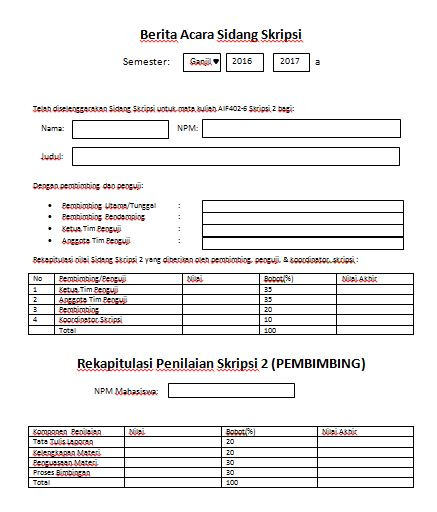
\includegraphics[scale=0.75]{Gambar/tampilan1}
		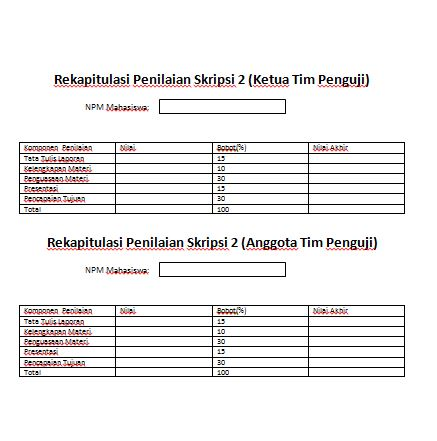
\includegraphics[scale=0.75]{Gambar/tampilan2}
		\caption{Perkiraan Tampilan}
		\label{fig:tampilan}
	\end{figure}